% =========================================================
\section{Contexto cinematográfico global (1965--1977)}
% =========================================================

El periodo comprendido entre 1965 y 1977 representa una fase de transformación radical del ecosistema cinematográfico mundial. La irrupción de nuevas formas de consumo audiovisual, la consolidación de la televisión como medio dominante, la crisis de los estudios clásicos en Estados Unidos y Europa, el ascenso de movimientos modernistas y contraculturales y la proliferación de cines de explotación contribuyeron a reconfigurar el mapa estético e industrial del cine internacional. Durante estos años se erosionan las bases del clasicismo fílmico, se redefinen los géneros y emergen nuevas sensibilidades que privilegian la subjetividad, el cuerpo, la fragmentación y la experimentación formal \citep{NowellSmith1996, Cook2007}. 

% ---------------------------------------------------------
\subsection{Transformaciones industriales y tecnológicas}
% ---------------------------------------------------------

A mediados de los sesenta, la televisión había alcanzado una presencia masiva en los principales mercados occidentales, reduciendo la asistencia a salas, forzando el cierre de cines y obligando a los estudios a reconfigurar sus estrategias de producción. En Estados Unidos, la asistencia anual cayó de unos 90 millones de espectadores semanales en 1948 a menos de 17 millones en 1967 \citep{Gomery1992}. Europa siguió un patrón similar, con descensos significativos en Francia, Italia y Reino Unido; por ejemplo, la asistencia británica se redujo de aproximadamente 1{,}400 millones de entradas en 1950 a 176 millones en 1965 \citep{Harper2004}. 

La industria respondió con diversas estrategias: generalización del color, formatos panorámicos y de gran formato (CinemaScope, 70 mm), cine espectáculo y, en el otro extremo, un aumento considerable de producciones de bajo presupuesto. Los mercados empezaron a polarizarse entre grandes producciones de estudio (épicos, musicales, cine catástrofe) y nichos de explotación (horror, erotismo, ciencia ficción menor), fenómeno que se observa tanto en Hollywood como en Italia, España, Francia o Alemania Occidental \citep{Hutchings2004, Klinger2006}.

Esta contracción de la asistencia se puede visualizar mediante la caída conjunta de los principales mercados occidentales:

\begin{figure}[t]
	\centering
	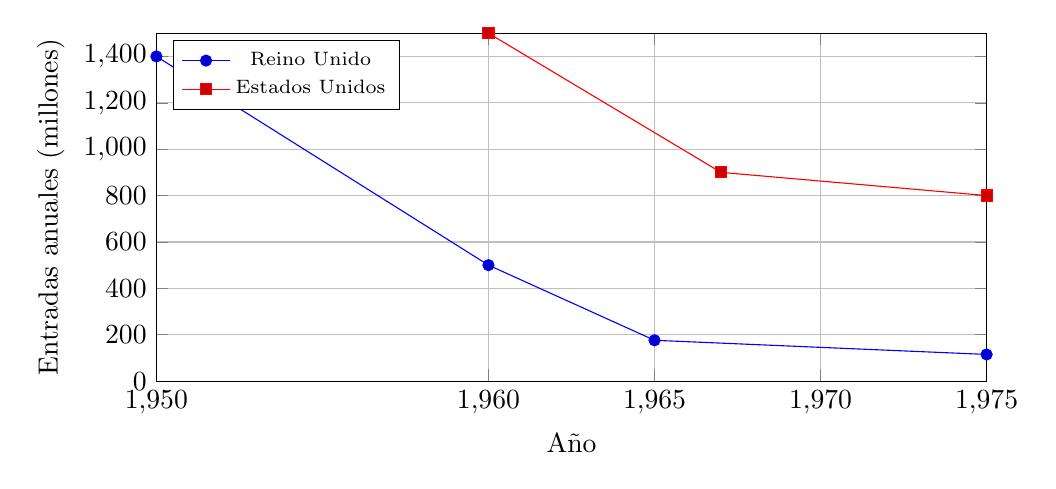
\begin{tikzpicture}
		\begin{axis}[
			width=\linewidth,
			height=6cm,
			xmin=1950, xmax=1975,
			ymin=0, ymax=1500,
			xlabel={Año},
			ylabel={Entradas anuales (millones)},
			xtick={1950,1960,1965,1970,1975},
			ytick={0,200,400,600,800,1000,1200,1400},
			grid=both,
			legend style={at={(0.02,0.98)},anchor=north west,font=\scriptsize},
			]
			% Reino Unido (datos aproximados)
			\addplot+[mark=*] coordinates {
				(1950,1400)
				(1960,500)
				(1965,176)
				(1975,115)
			};
			\addlegendentry{Reino Unido}
			
			% Estados Unidos (entradas semanales transformadas a millones anuales aprox.)
			\addplot+[mark=square*] coordinates {
				(1950,3000)
				(1960,1500)
				(1967,900)
				(1975,800)
			};
			\addlegendentry{Estados Unidos}
		\end{axis}
	\end{tikzpicture}
	\caption{Descenso de la asistencia cinematográfica en EE.\,UU. y Reino Unido (1950--1975). Datos aproximados a partir de \cite{Gomery1992, Harper2004}.}
	\label{fig:global_admissions_plot}
\end{figure}

Aunque las cifras de la figura \ref{fig:global_admissions_plot} son aproximadas, ilustran una tendencia clara: el cine deja de ser el medio hegemónico de entretenimiento masivo y se ve obligado a repensar su modelo de negocio ante la competencia de la televisión y, hacia finales de los setenta, del vídeo doméstico emergente.

% ---------------------------------------------------------
\subsection{Movimientos modernistas y contraculturales}
% ---------------------------------------------------------

El período 1965--1977 coincide con el auge global del cine modernista, que redefinió el lenguaje fílmico mediante fragmentación narrativa, reflexividad, subjetividad extrema y rupturas espaciales y temporales. La Nouvelle Vague seguía produciendo obras clave —como \emph{Pierrot le fou} (Godard, 1965) o \emph{La Chinoise} (Godard, 1967)— que exploraban la relación entre política, juventud y medios de comunicación. En Italia, Antonioni continuó la investigación de la alienación moderna con \emph{Blow-Up} (1966) y \emph{Zabriskie Point} (1970). En Alemania, el Nuevo Cine Alemán consolidó figuras como Fassbinder (\emph{Liebe ist kälter als der Tod}, 1969), Herzog (\emph{Aguirre, der Zorn Gottes}, 1972) y Wenders (\emph{Der amerikanische Freund}, 1977) \citep{Elsaesser1989}.

Fuera de Europa, el modernismo cinematográfico adoptó formas específicas: el Cinema Novo brasileño de Glauber Rocha, el cine político latinoamericano, el cine de autor japonés de Ōshima y Yoshida, o el trabajo de cineastas africanos como Sembène. Todos estos movimientos compartían un interés por la desestabilización del realismo, la exploración de estados psicogeográficos y la crítica cultural; un horizonte que dialoga, aunque desde coordenadas distintas, con el anti-realismo y la imaginería pop-publicitaria que Obayashi desarrollaría en \textit{Hausu}.

% ---------------------------------------------------------
\subsection{Géneros populares y cines de explotación}
% ---------------------------------------------------------

Simultáneamente, la década vio una proliferación internacional de cines populares y de explotación, frecuentemente producidos con bajo presupuesto y dirigidos a públicos juveniles. Italia desarrolló el \emph{giallo} (Argento, \emph{L'uccello dalle piume di cristallo}, 1970), los \emph{poliziotteschi} (\emph{La polizia incrimina, la legge assolve}, Lenzi, 1973) y el horror gótico tardío. Reino Unido impulsó el horror de la Hammer (\emph{Dracula Has Risen from the Grave}, 1968). Estados Unidos consolidó el \emph{exploitation cinema} con obras como \emph{Night of the Living Dead} (Romero, 1968), \emph{The Last House on the Left} (Craven, 1972) y la ola blaxploitation (\emph{Shaft}, Parks, 1971) \citep{Hutchings2004, Koven2006}. 

En este panorama, el cuerpo —fragmentado, estilizado, mutilado o erotizado— se convirtió en un espacio de experimentación estética. El auge del cine pornográfico industrial tras \emph{Deep Throat} (Damiano, 1972) reafirmó una tendencia global hacia la espectacularización del cuerpo, que resonaba de forma distinta en Japón con el \emph{Pinku Eiga} y posteriormente con los \emph{Roman Porno}. Zahlten y Sharp han mostrado cómo estos circuitos de explotación sexual funcionaron como verdaderos laboratorios formales y económicos en paralelo a las producciones de prestigio \citep{Sharp2011, Zahlten2017}.

% ---------------------------------------------------------
\subsection{Crisis del viejo Hollywood y emergencia del New Hollywood}
% ---------------------------------------------------------

La quiebra del sistema clásico estadounidense entre 1967 y 1975 produjo una renovación profunda en los modos de producción y narración. Tras los fracasos millonarios de \emph{Cleopatra} (1963) y \emph{Doctor Dolittle} (1967), los estudios cedieron espacio a jóvenes cineastas formados en escuelas de cine (Coppola, Scorsese, Altman, De Palma), cuyas obras incorporaron violencia estilizada, ambigüedad moral y crítica sociopolítica: \emph{Bonnie and Clyde} (Penn, 1967), \emph{The Graduate} (Nichols, 1967), \emph{Easy Rider} (Hopper, 1969), \emph{Mean Streets} (Scorsese, 1973) o \emph{Carrie} (De Palma, 1976). 

Schatz y Cook han descrito esta fase como un \enquote{interregno} entre el sistema clásico de estudios y el posterior régimen del blockbuster, marcado por presupuestos relativamente moderados, fuerte presencia de personajes marginales y temas contemporáneos, y una mayor autonomía de los directores dentro de los grandes estudios \citep{Schatz1993, Cook2007}. Este clima de libertad expresiva y experimentación formal configura un marco global convergente con los procesos paralelos en Japón, donde la crisis del \textit{studio system} abrió espacios para propuestas híbridas como \emph{Hausu}.

% ---------------------------------------------------------
\subsection{\emph{Jaws} (1975) y el nacimiento del blockbuster global}
% ---------------------------------------------------------

El lanzamiento de \emph{Jaws} (Spielberg, 1975) transformó de forma irreversible el modelo económico del cine comercial internacional. Con un presupuesto estimado en torno a 7--9 millones de dólares y una recaudación mundial que superó los 470 millones, la película se convirtió en el mayor éxito de taquilla de la historia hasta entonces \citep{Wyatt1994, Prince2000}. Más allá de las cifras, su importancia radica en el modelo de distribución y marketing que consolidó: estreno veraniego, campaña televisiva intensiva, lanzamiento simultáneo en cientos de salas y una fuerte explotación de productos derivados.

Wyatt caracteriza \emph{Jaws} como prototipo del \enquote{high concept film}: una premisa fácilmente resumible (\enquote{un tiburón asesino aterroriza una localidad costera}), iconografía poderosa (el póster del tiburón emergiendo bajo la nadadora), y un diseño pensado para generar imágenes reutilizables en tráilers, anuncios y merchandising \citep{Wyatt1994}. Prince subraya que el film combinaba la herencia del cine de autor (uso del fuera de campo, construcción del suspense, tratamiento del trauma comunitario) con una estructura narrativa clásica y un dispositivo de estrellas y efectos especiales que lo hacían accesible al gran público \citep{Prince2000}.

En términos de tendencias industriales, \emph{Jaws} marca el inicio de un desplazamiento del modelo de \emph{roadshow} (estrenos limitados que se expanden lentamente) hacia la llamada \enquote{saturation booking}: un gran número de copias en estreno simultáneo nacional, apoyado en una campaña publicitaria masiva, con el objetivo de maximizar la recaudación en las primeras semanas antes de que opere el boca a boca negativo. Este modelo será perfeccionado dos años después con \emph{Star Wars} (Lucas, 1977) y se convertirá en la norma del blockbuster global en los años ochenta \citep{Schatz1993, Klinger2006}.

El impacto de \emph{Jaws} no se limitó a Estados Unidos. Los análisis de Klinger y de Thompson y Bordwell muestran cómo el éxito del film reconfiguró las expectativas de taquilla en mercados europeos y asiáticos: los distribuidores exigían cada vez más productos capaces de sostener campañas sincronizadas y de generar fenómenos de audiencia concentrados \citep{Klinger2006, BordwellThompson2003}. En Japón, Toho y otros estudios observaron con atención el rendimiento de estos nuevos \emph{event films}. La importación de \emph{Jaws} y, poco después, de \emph{Star Wars} demostró que los blockbusters estadounidenses podían desplazar del primer plano a las producciones nacionales en términos de visibilidad y recaudación, intensificando la sensación de crisis estructural ya presente en el sistema japonés.

En este contexto, \textit{Hausu} puede entenderse como una respuesta local a la lógica del blockbuster global, pero desde una posición lateral. Toho no podía competir con los presupuestos ni con la infraestructura promocional de Spielberg o Lucas, pero sí podía intentar capturar la atención del mismo público juvenil mediante una combinación de terror, humor y espectáculo visual intenso. \textit{Hausu} comparte con \emph{Jaws} ciertos rasgos del cine de evento —un concepto llamativo, una fuerte explotación visual de la casa como dispositivo de muerte, un uso agresivo de los efectos especiales—, pero los desplaza hacia un territorio abiertamente experimental, más cercano a la cultura del anuncio televisivo, el \textit{shōjo manga} y el cine de vanguardia que al clasicismo renovado del New Hollywood.

Así, la hibridez estética de \textit{Hausu} no solo responde a la crisis interna del cine japonés, sino también a la necesidad de negociar con un mercado global en el que el modelo del blockbuster estadounidense se imponía como forma dominante de producción, distribución y consumo cinematográfico.
